\documentclass[12pt]{article}
\usepackage[utf8]{inputenc}
\usepackage[letterpaper, margin=0.5in, headheight=10pt]{geometry}
\usepackage{amsmath}
\usepackage{amssymb}
\usepackage{graphicx}
\usepackage{pdflscape}

\newcommand\figWidth{4in}
\newcommand\figWidthLarge{9.5in}

\begin{document}
    \begin{landscape}
    \begin{figure}
        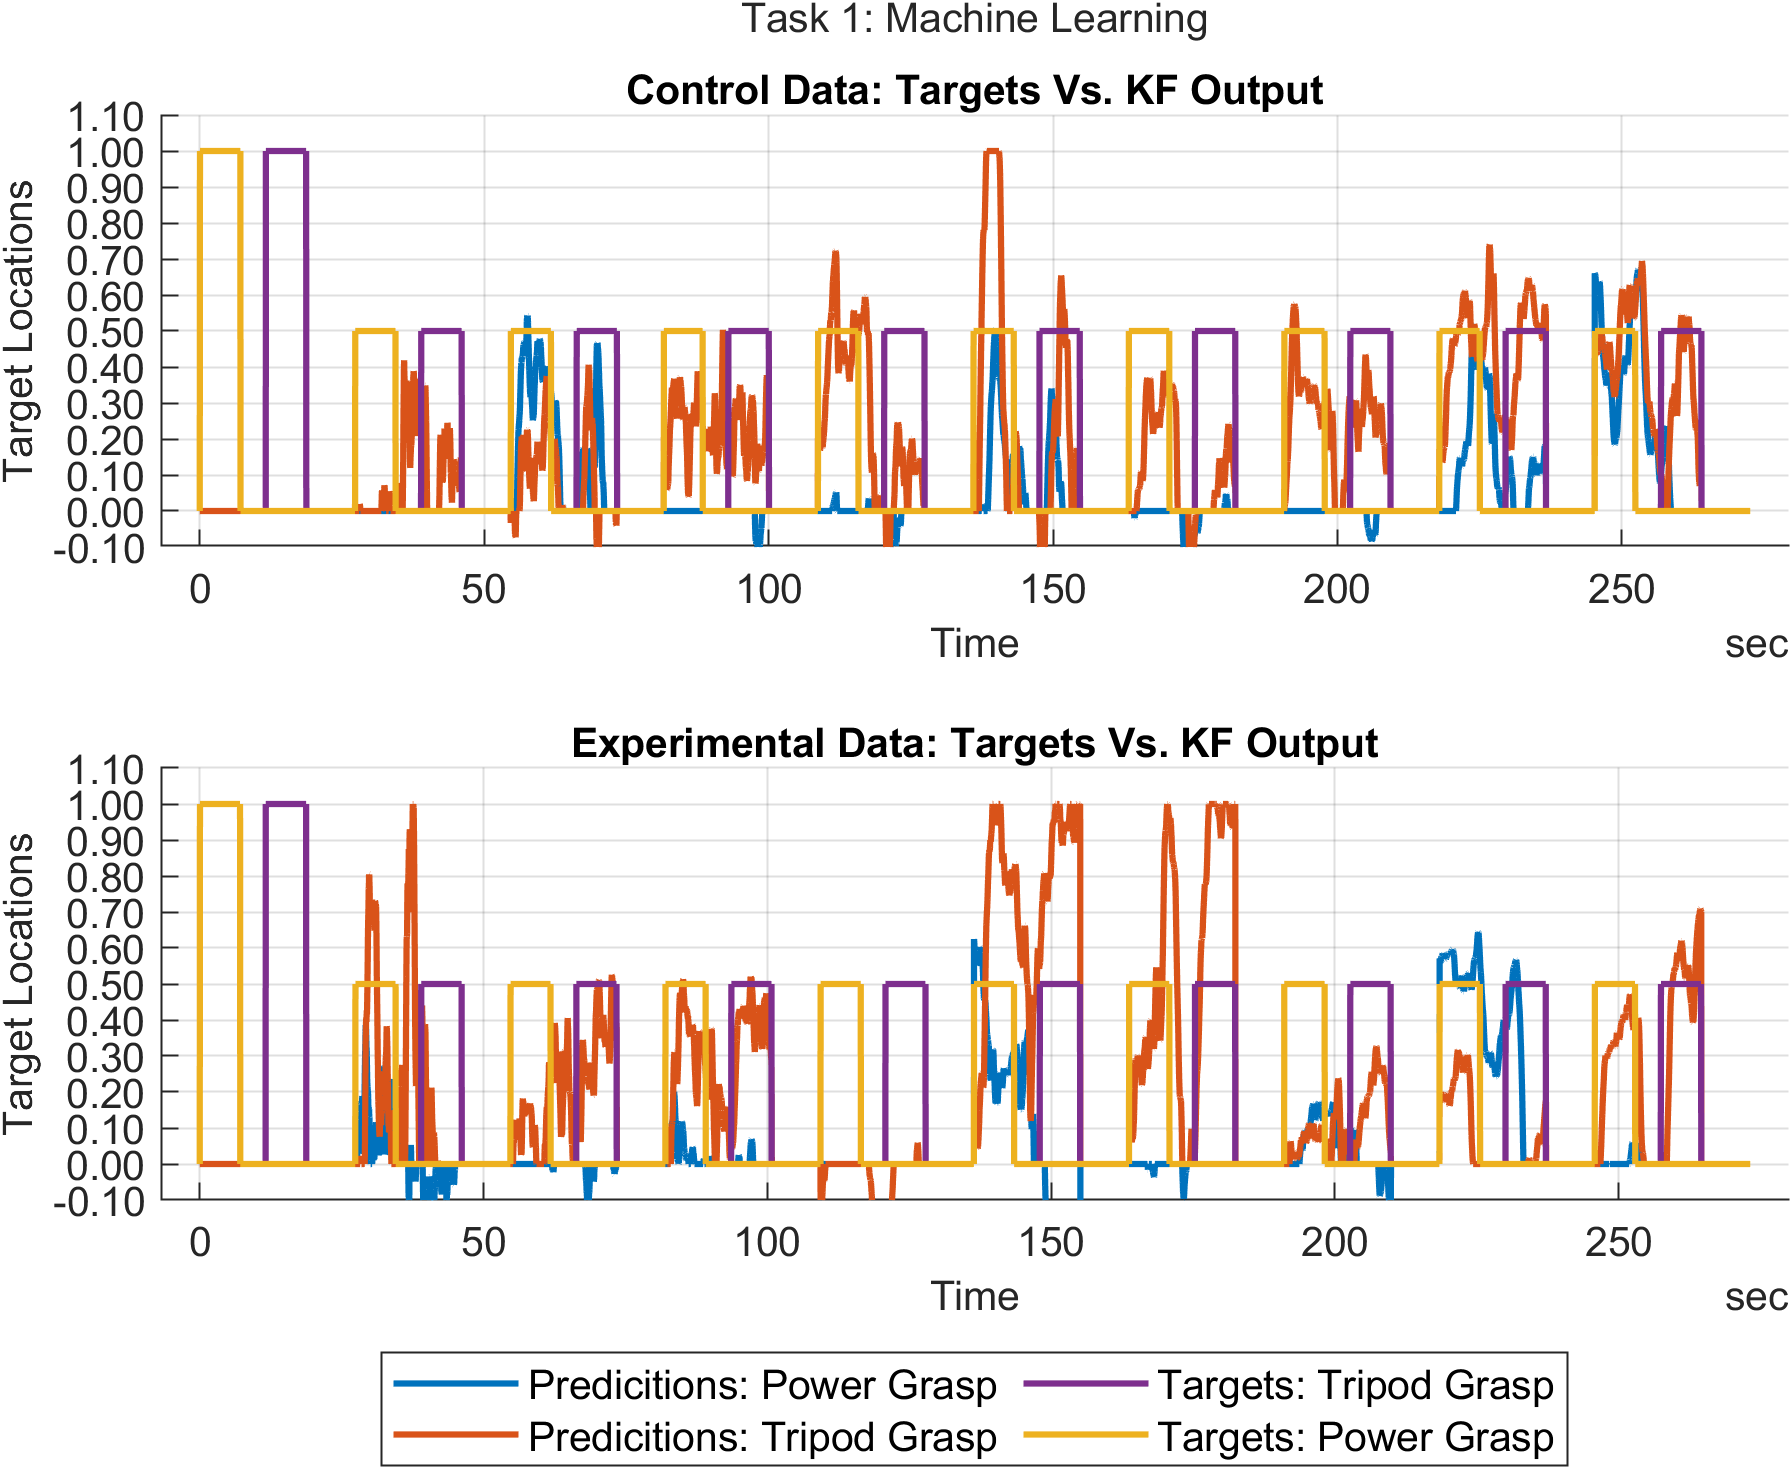
\includegraphics[width = \figWidthLarge]{t1-kf-out.png}
    \end{figure}
    \end{landscape}
    \newpage \clearpage
    
    \begin{figure}
        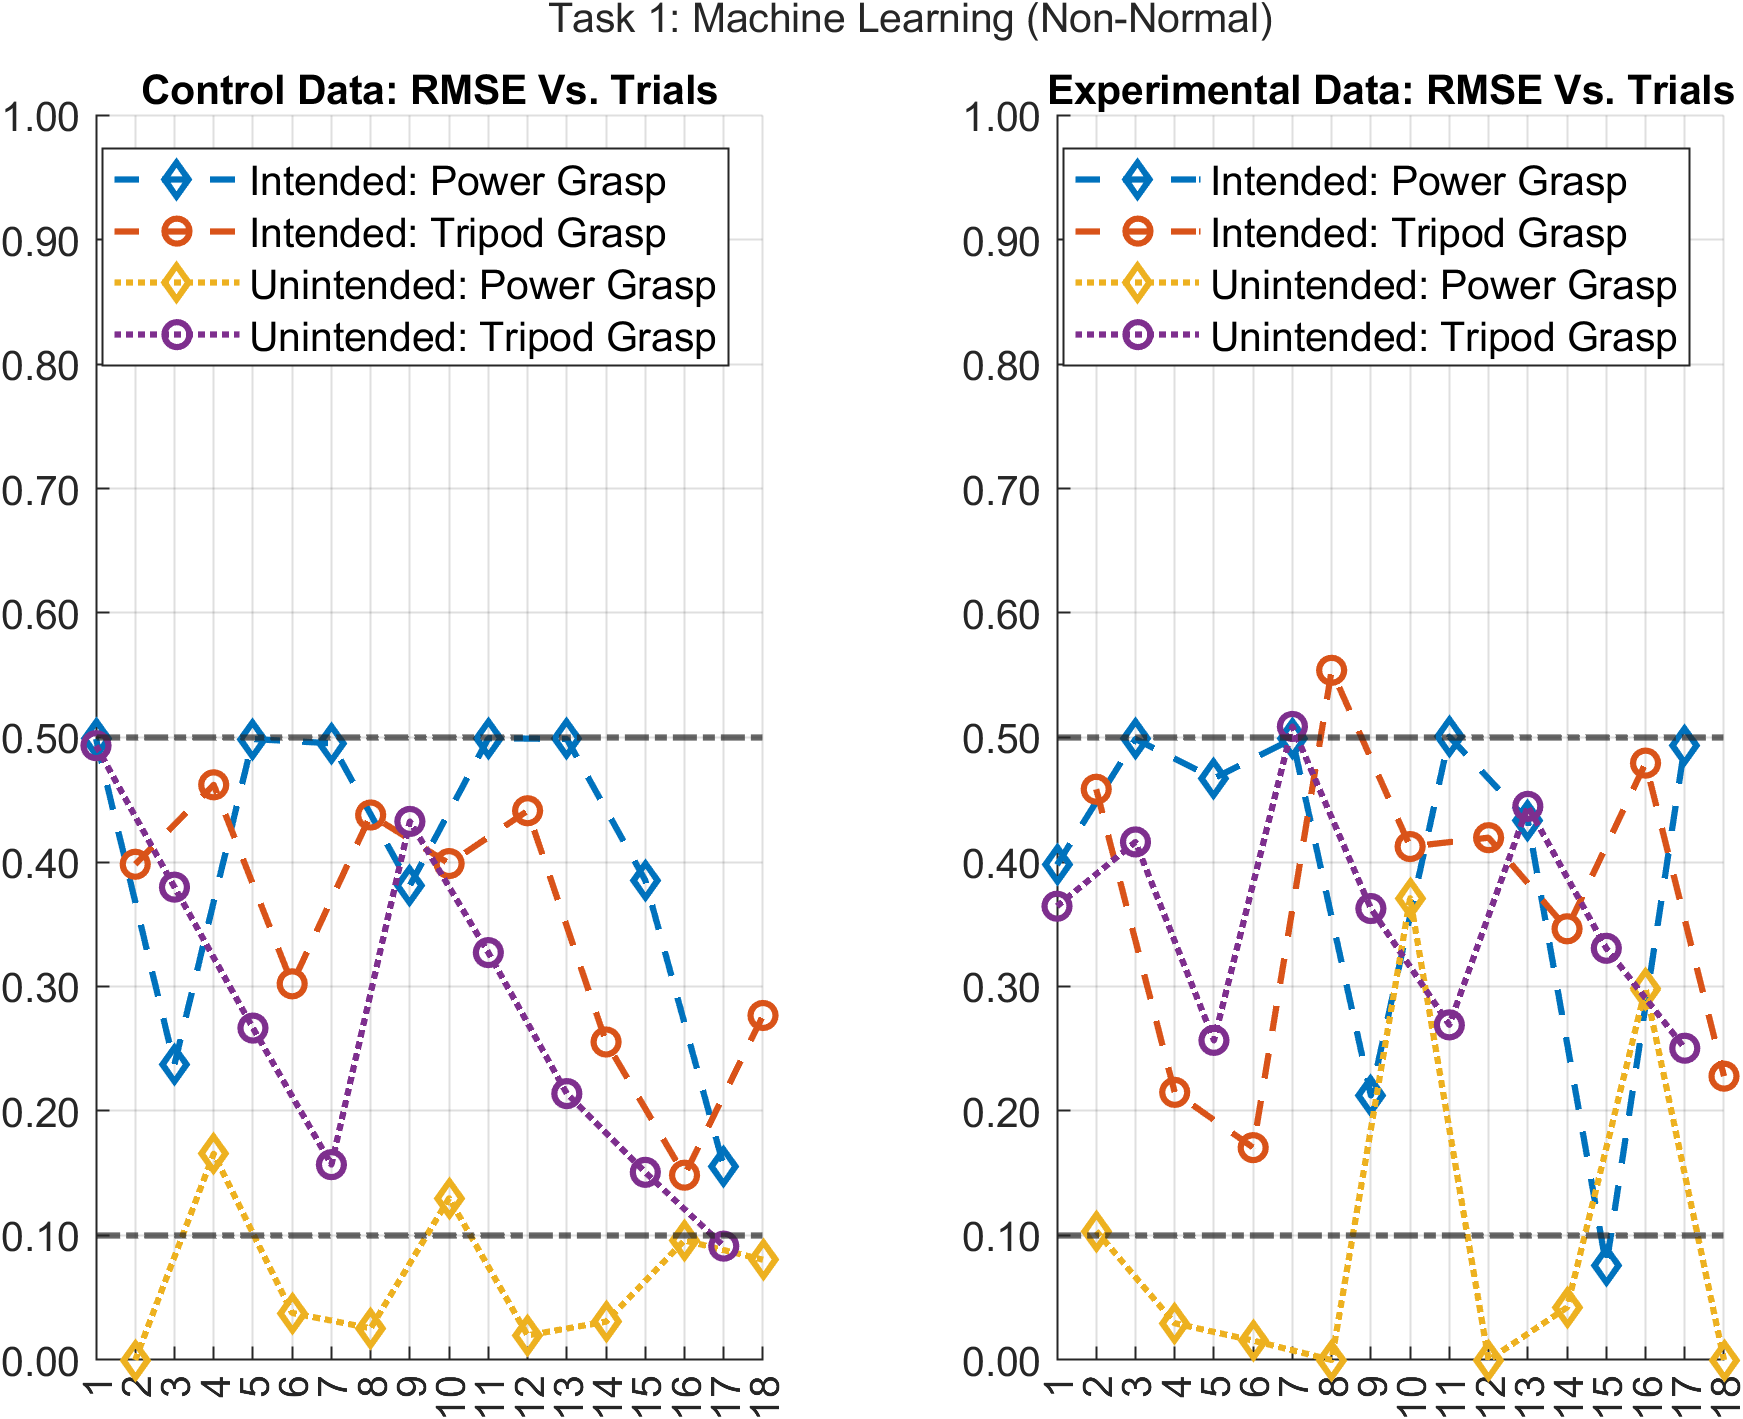
\includegraphics[width = \figWidth]{t1-rmse-xnorm.png}
    \end{figure}
    \begin{figure}
        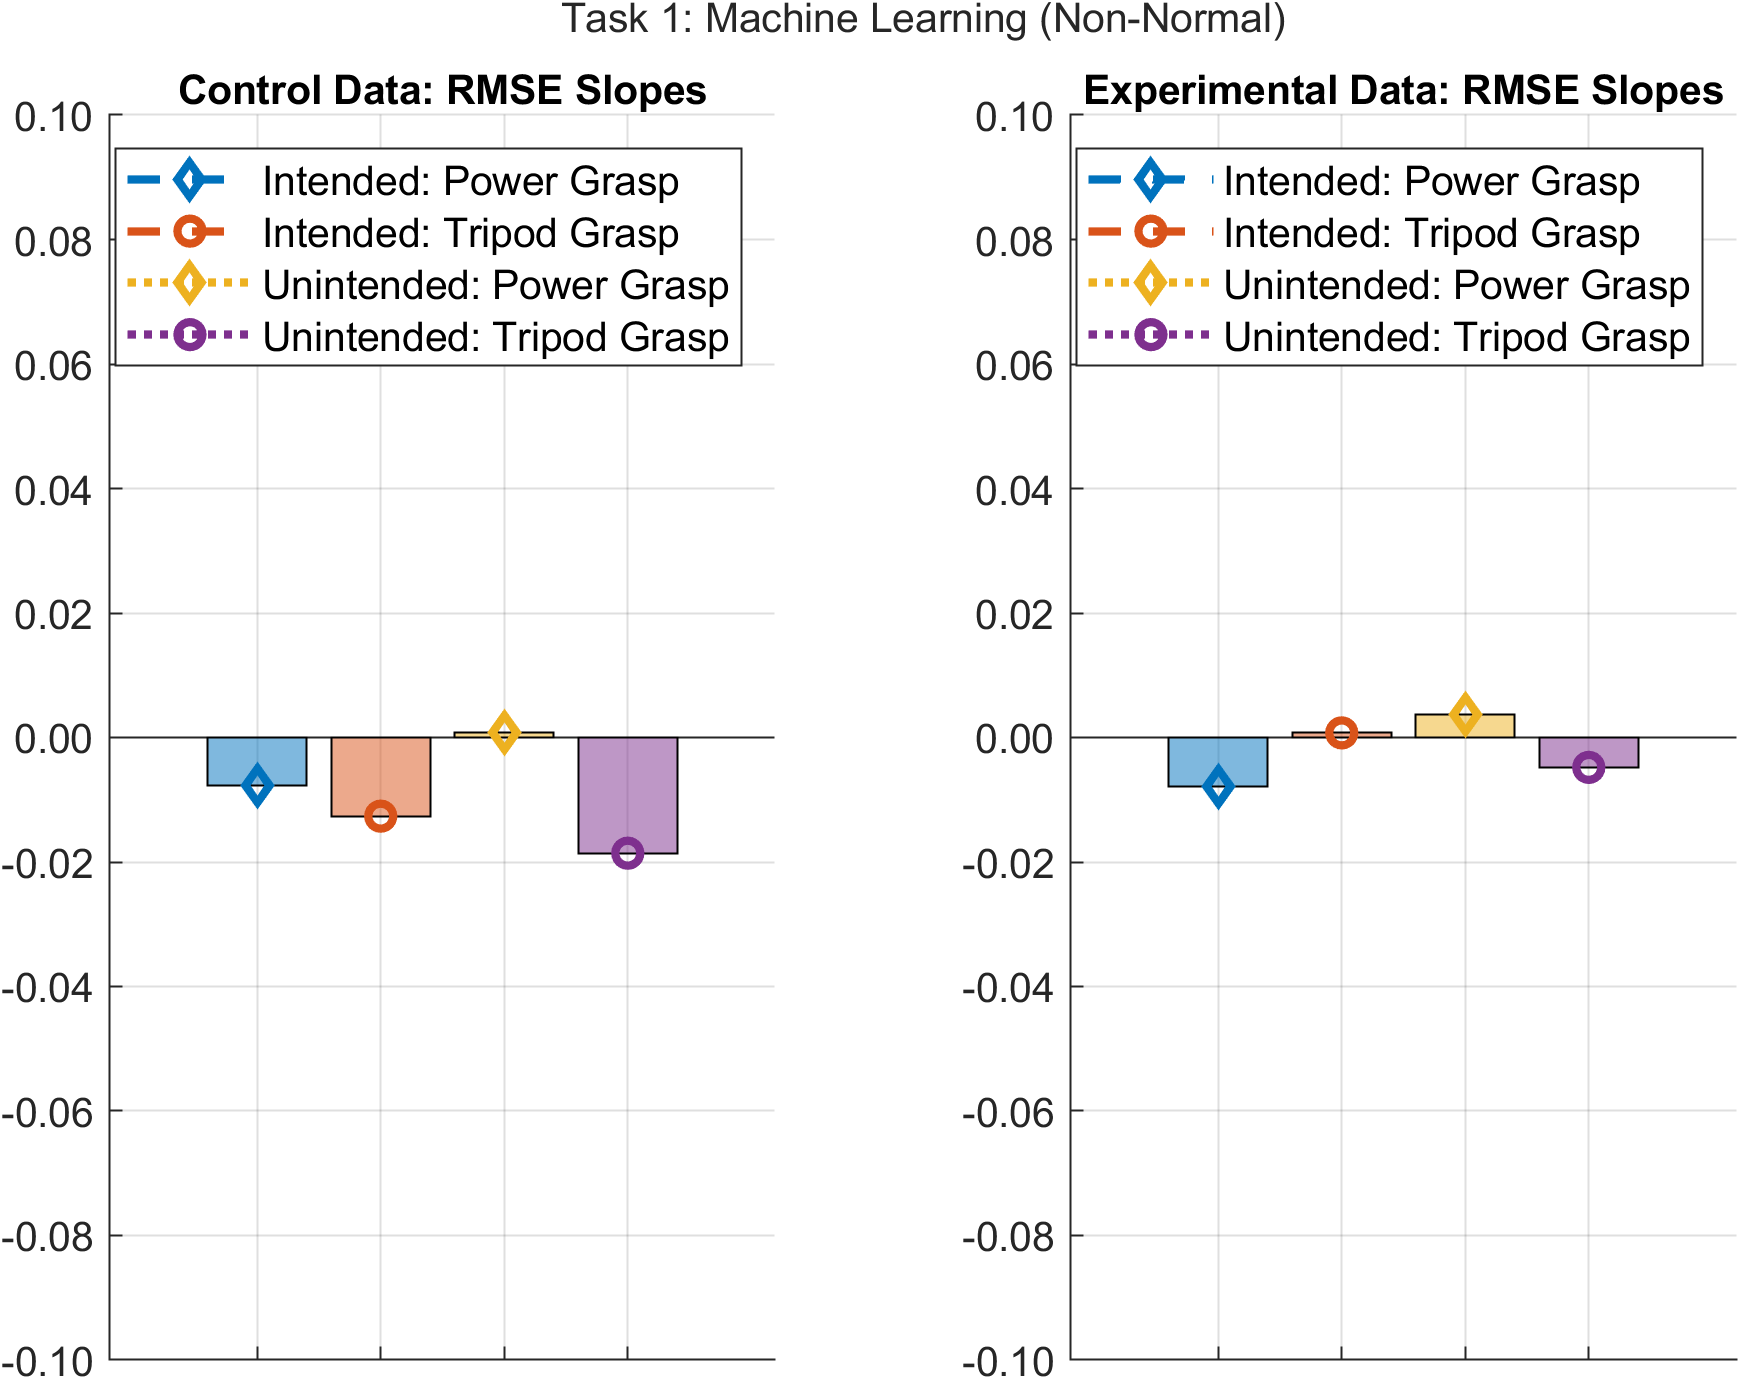
\includegraphics[width = \figWidth]{t1-bar-xnorm.png}
    \end{figure}
    \begin{figure}
        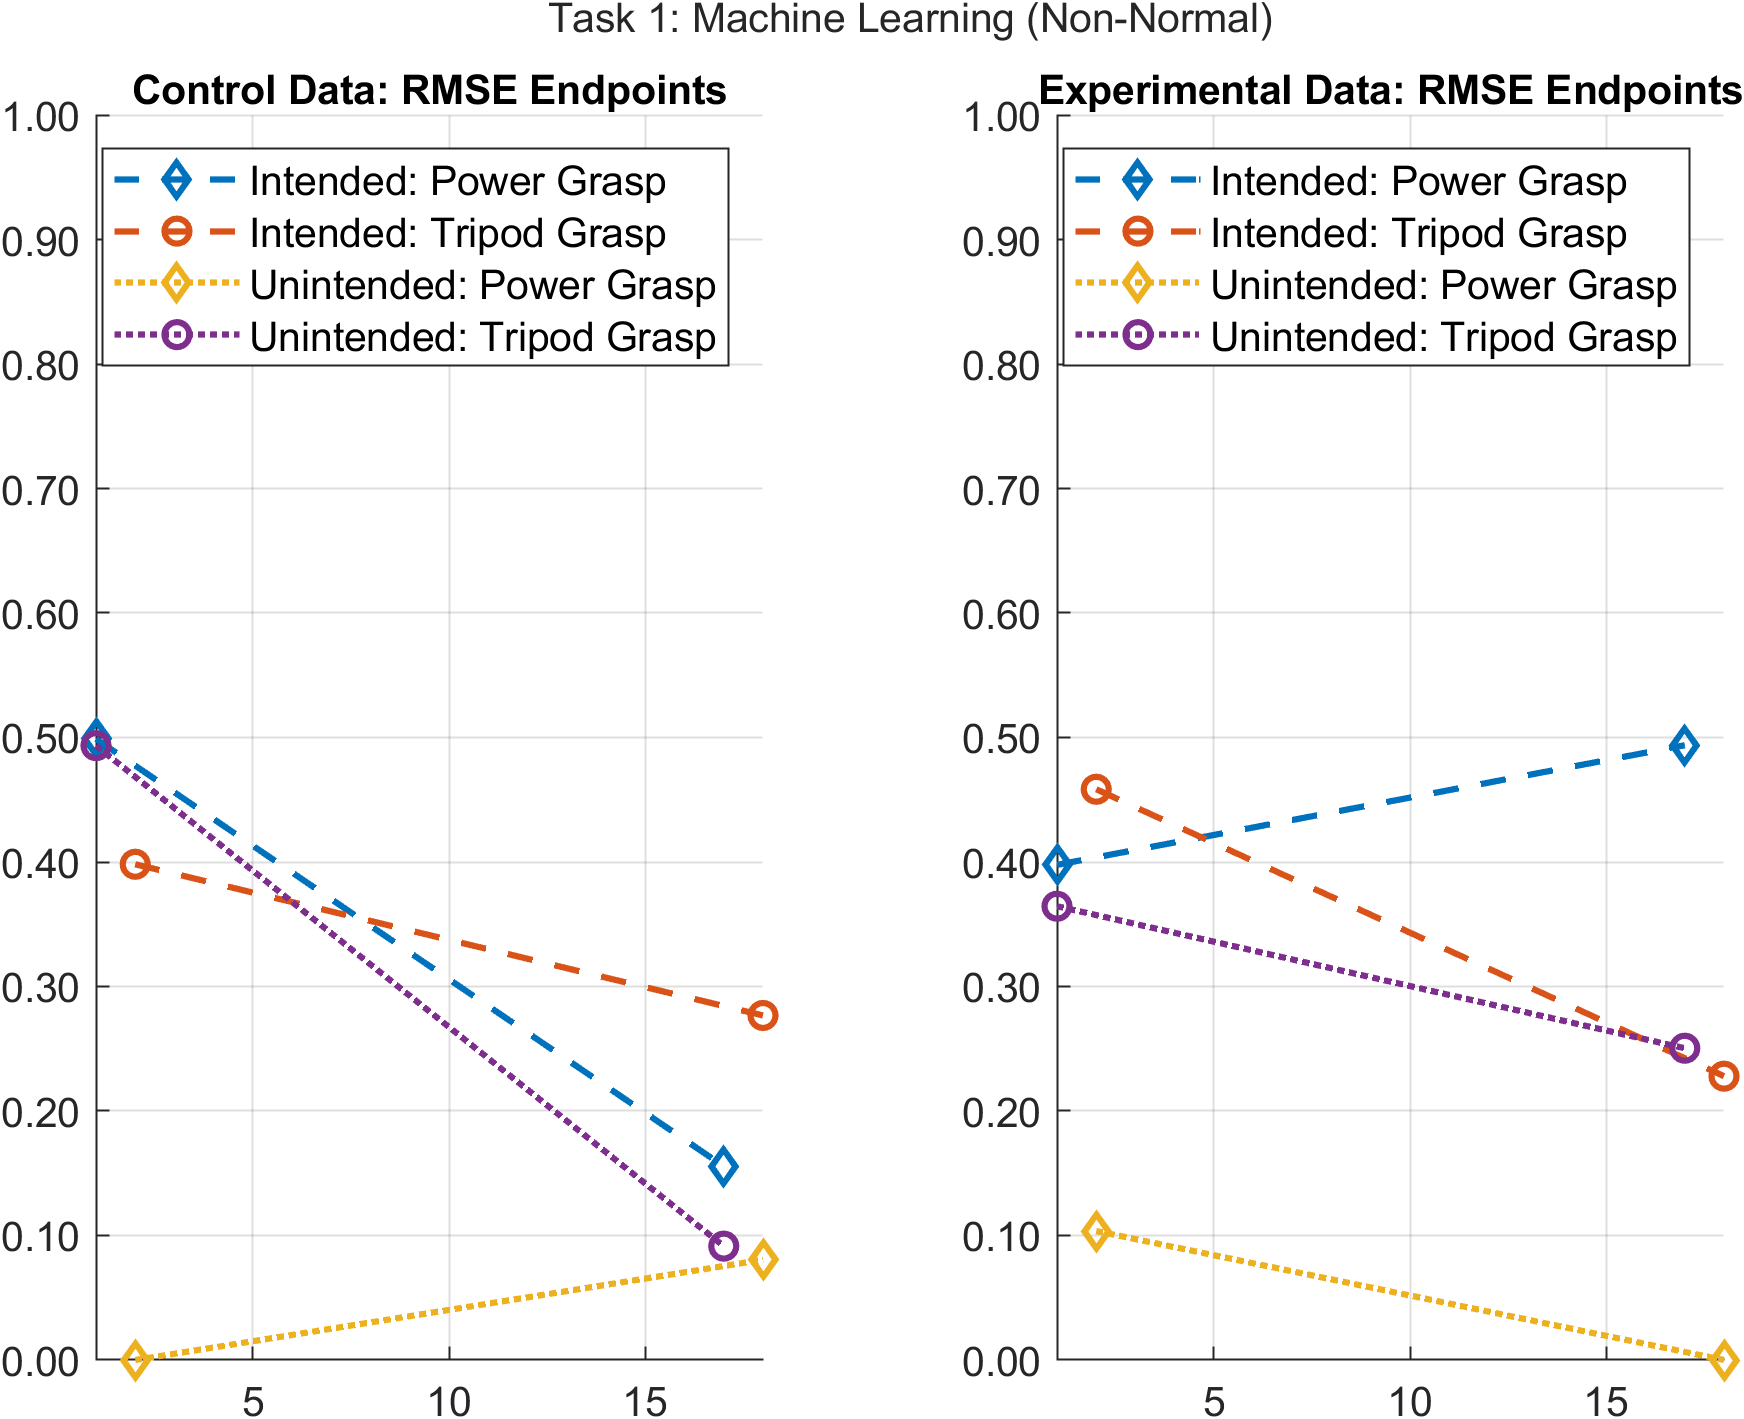
\includegraphics[width = \figWidth]{t1-spaghetti-xnorm.png}
    \end{figure}

    \newpage \clearpage
    %%%%%%%%%%%%%%%%%%%
    \begin{landscape}
    \begin{figure}
        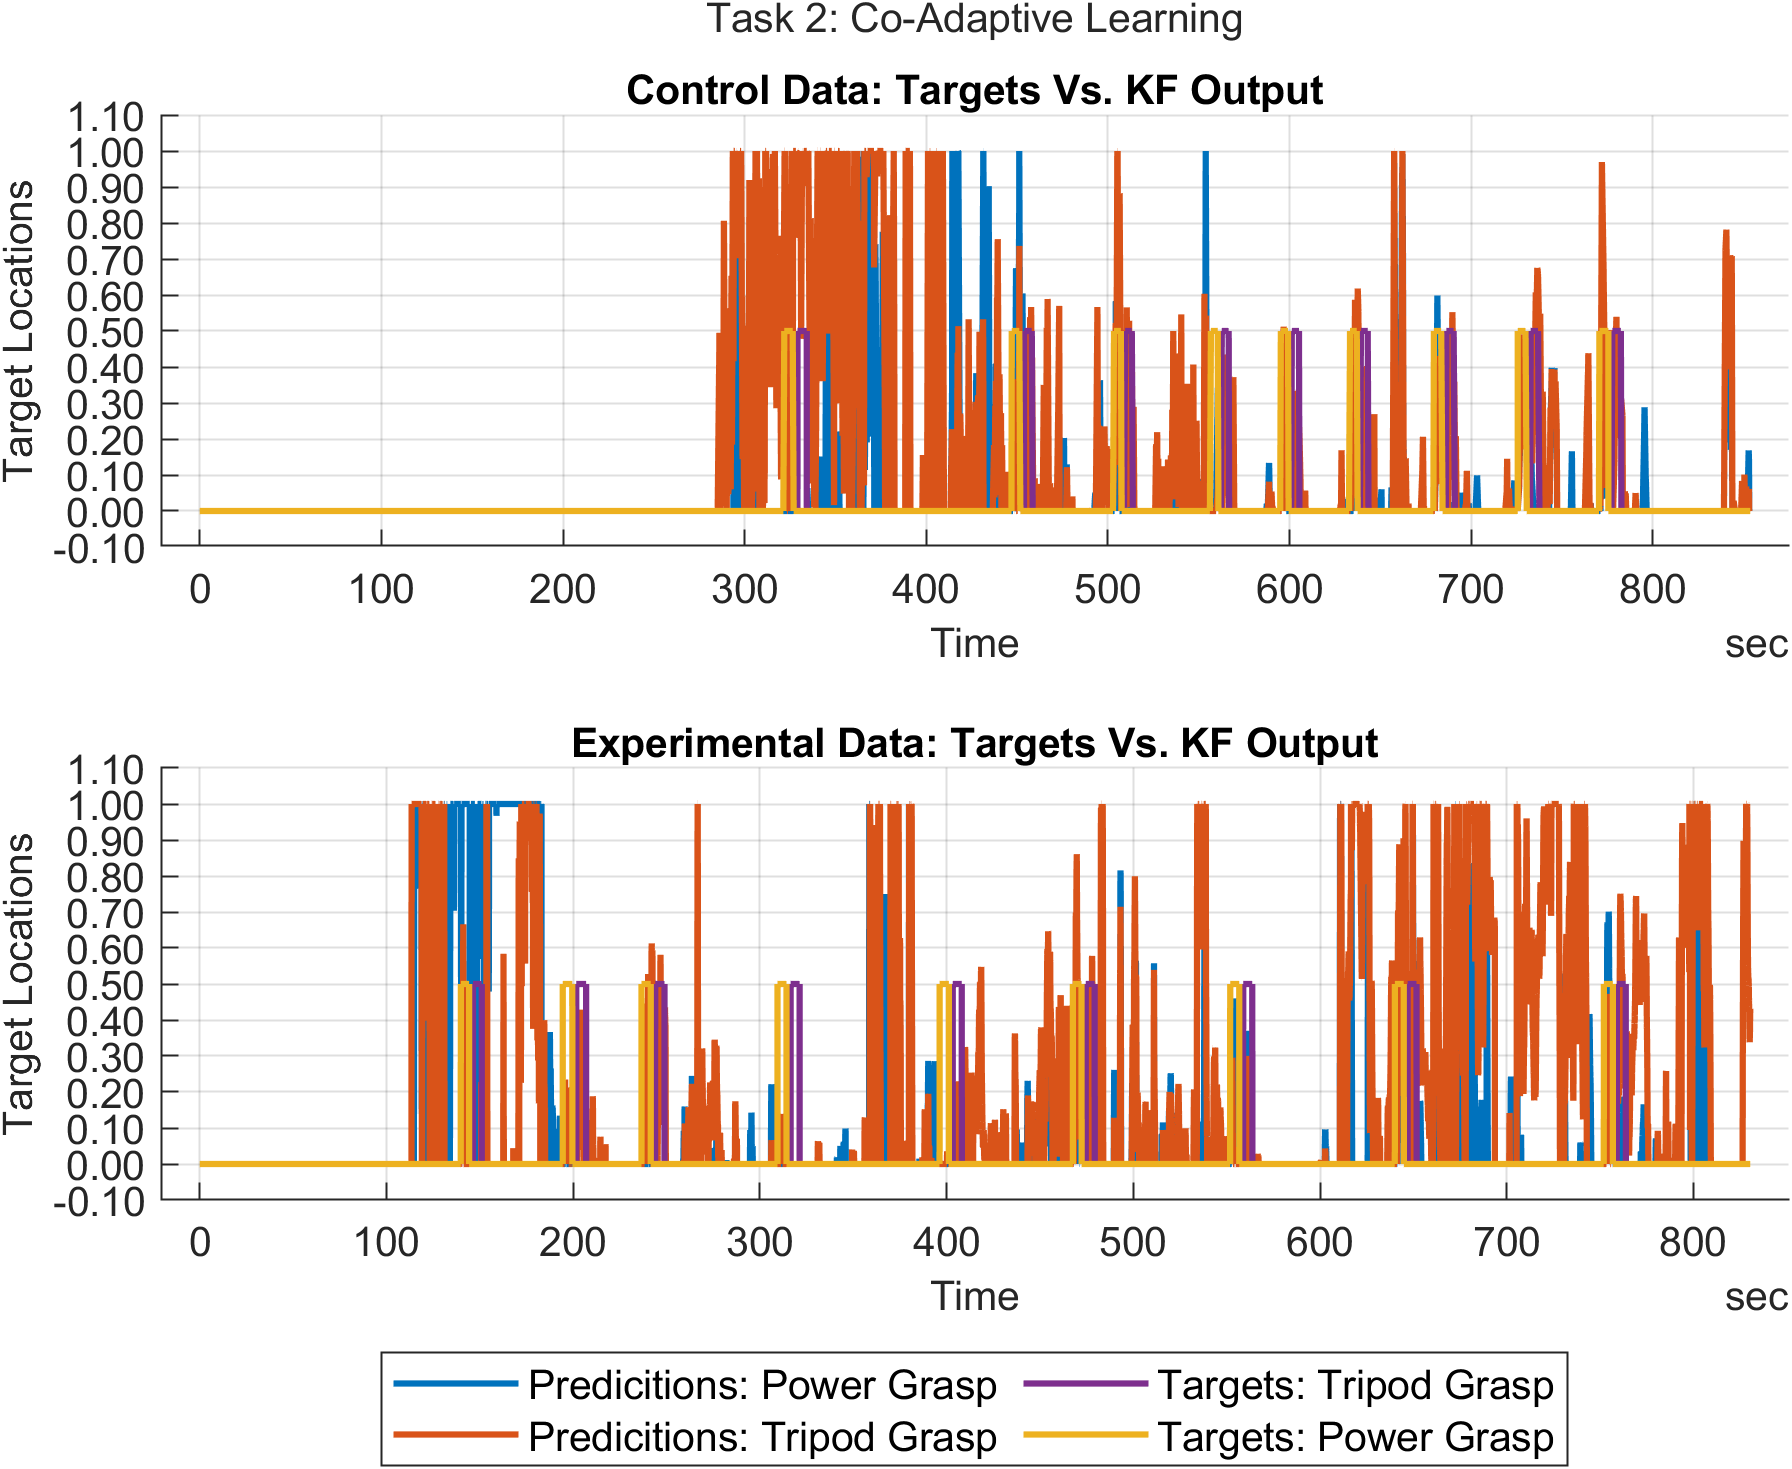
\includegraphics[width = \figWidthLarge]{t2-kf-out.png}
    \end{figure}
    \end{landscape}
    \newpage \clearpage
    \begin{figure}
        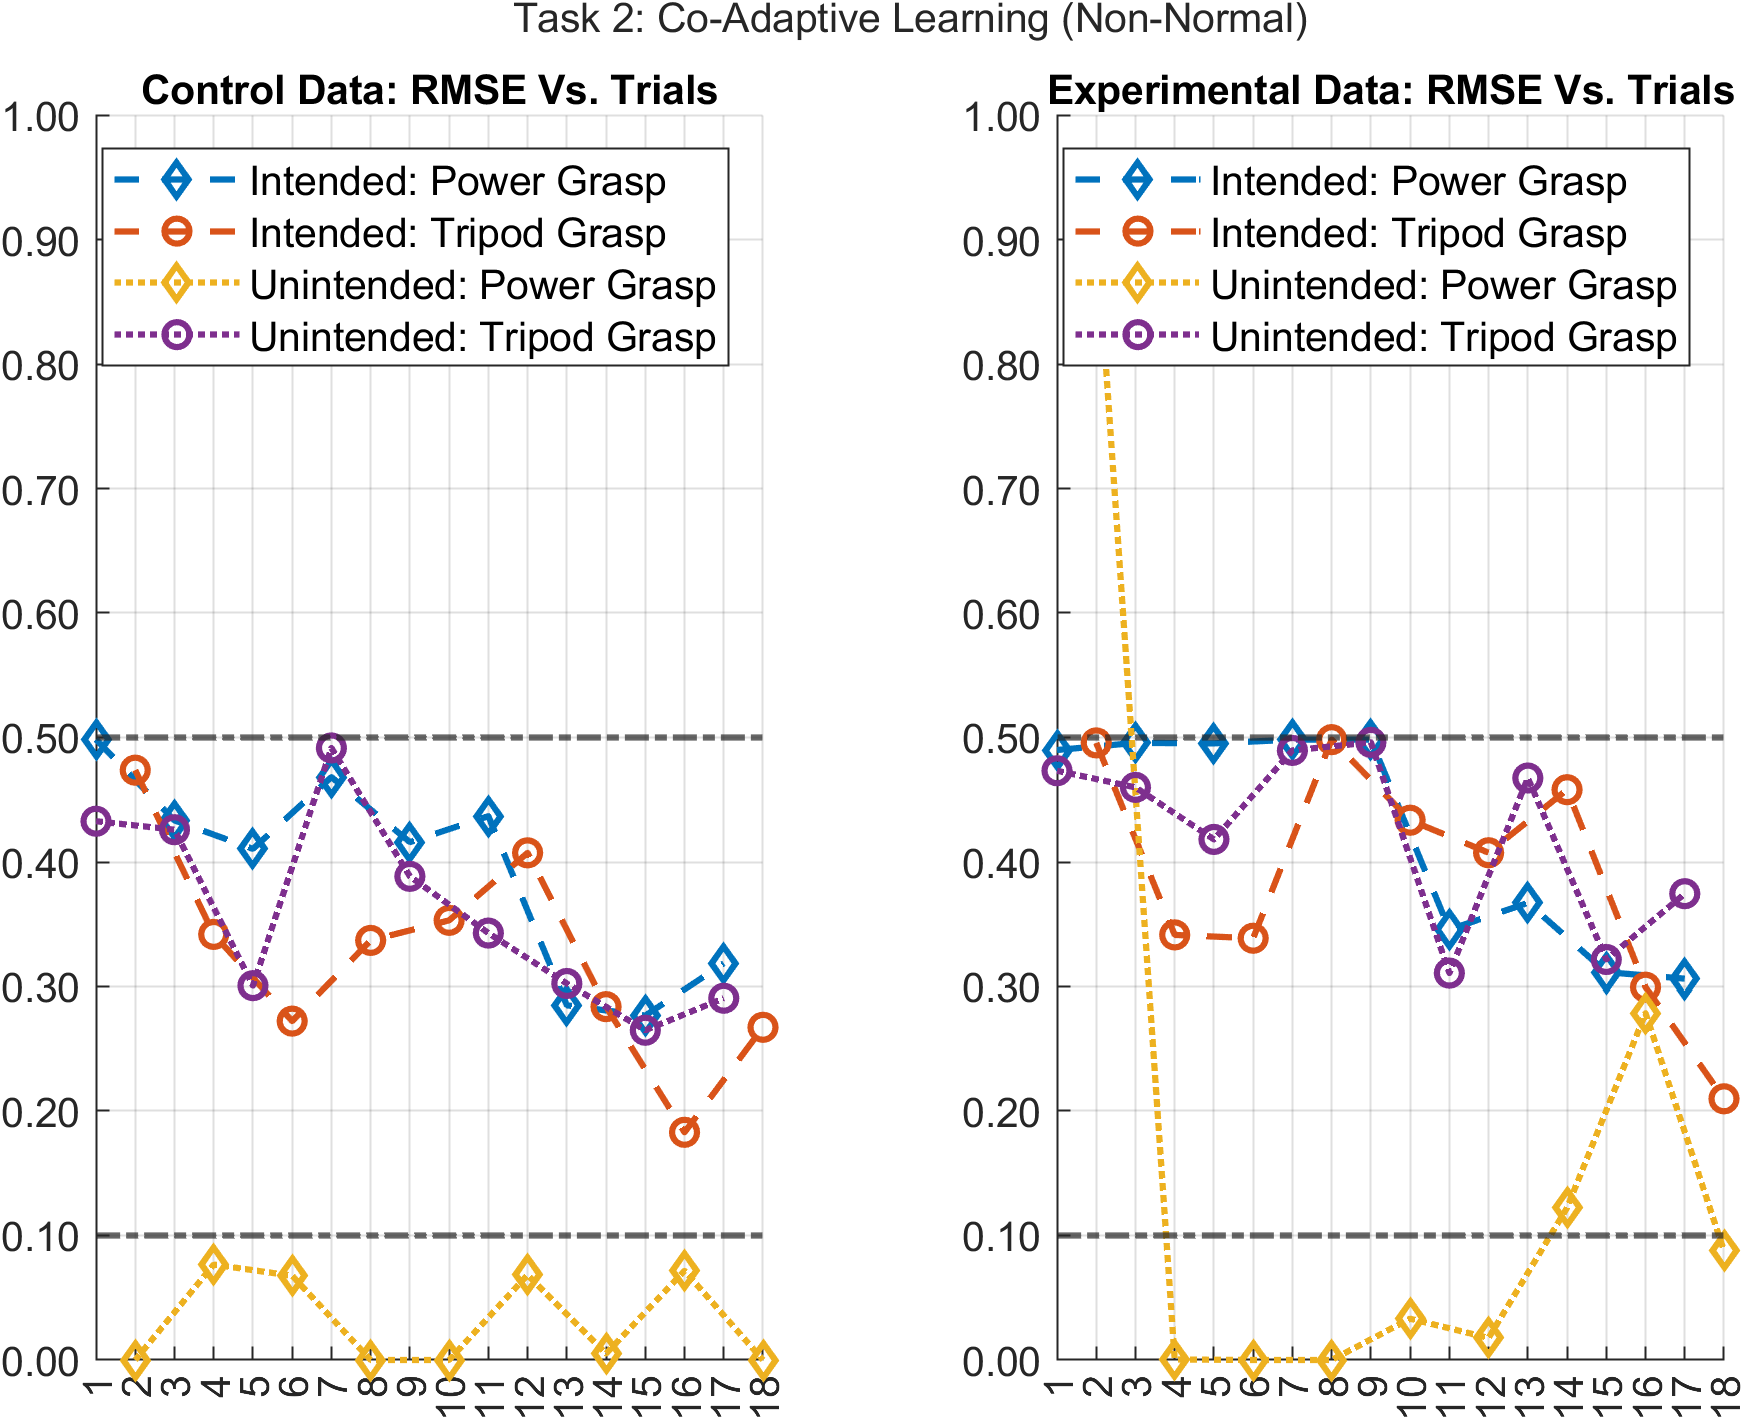
\includegraphics[width = \figWidth]{t2-rmse-xnorm.png}
    \end{figure}
    \begin{figure}
        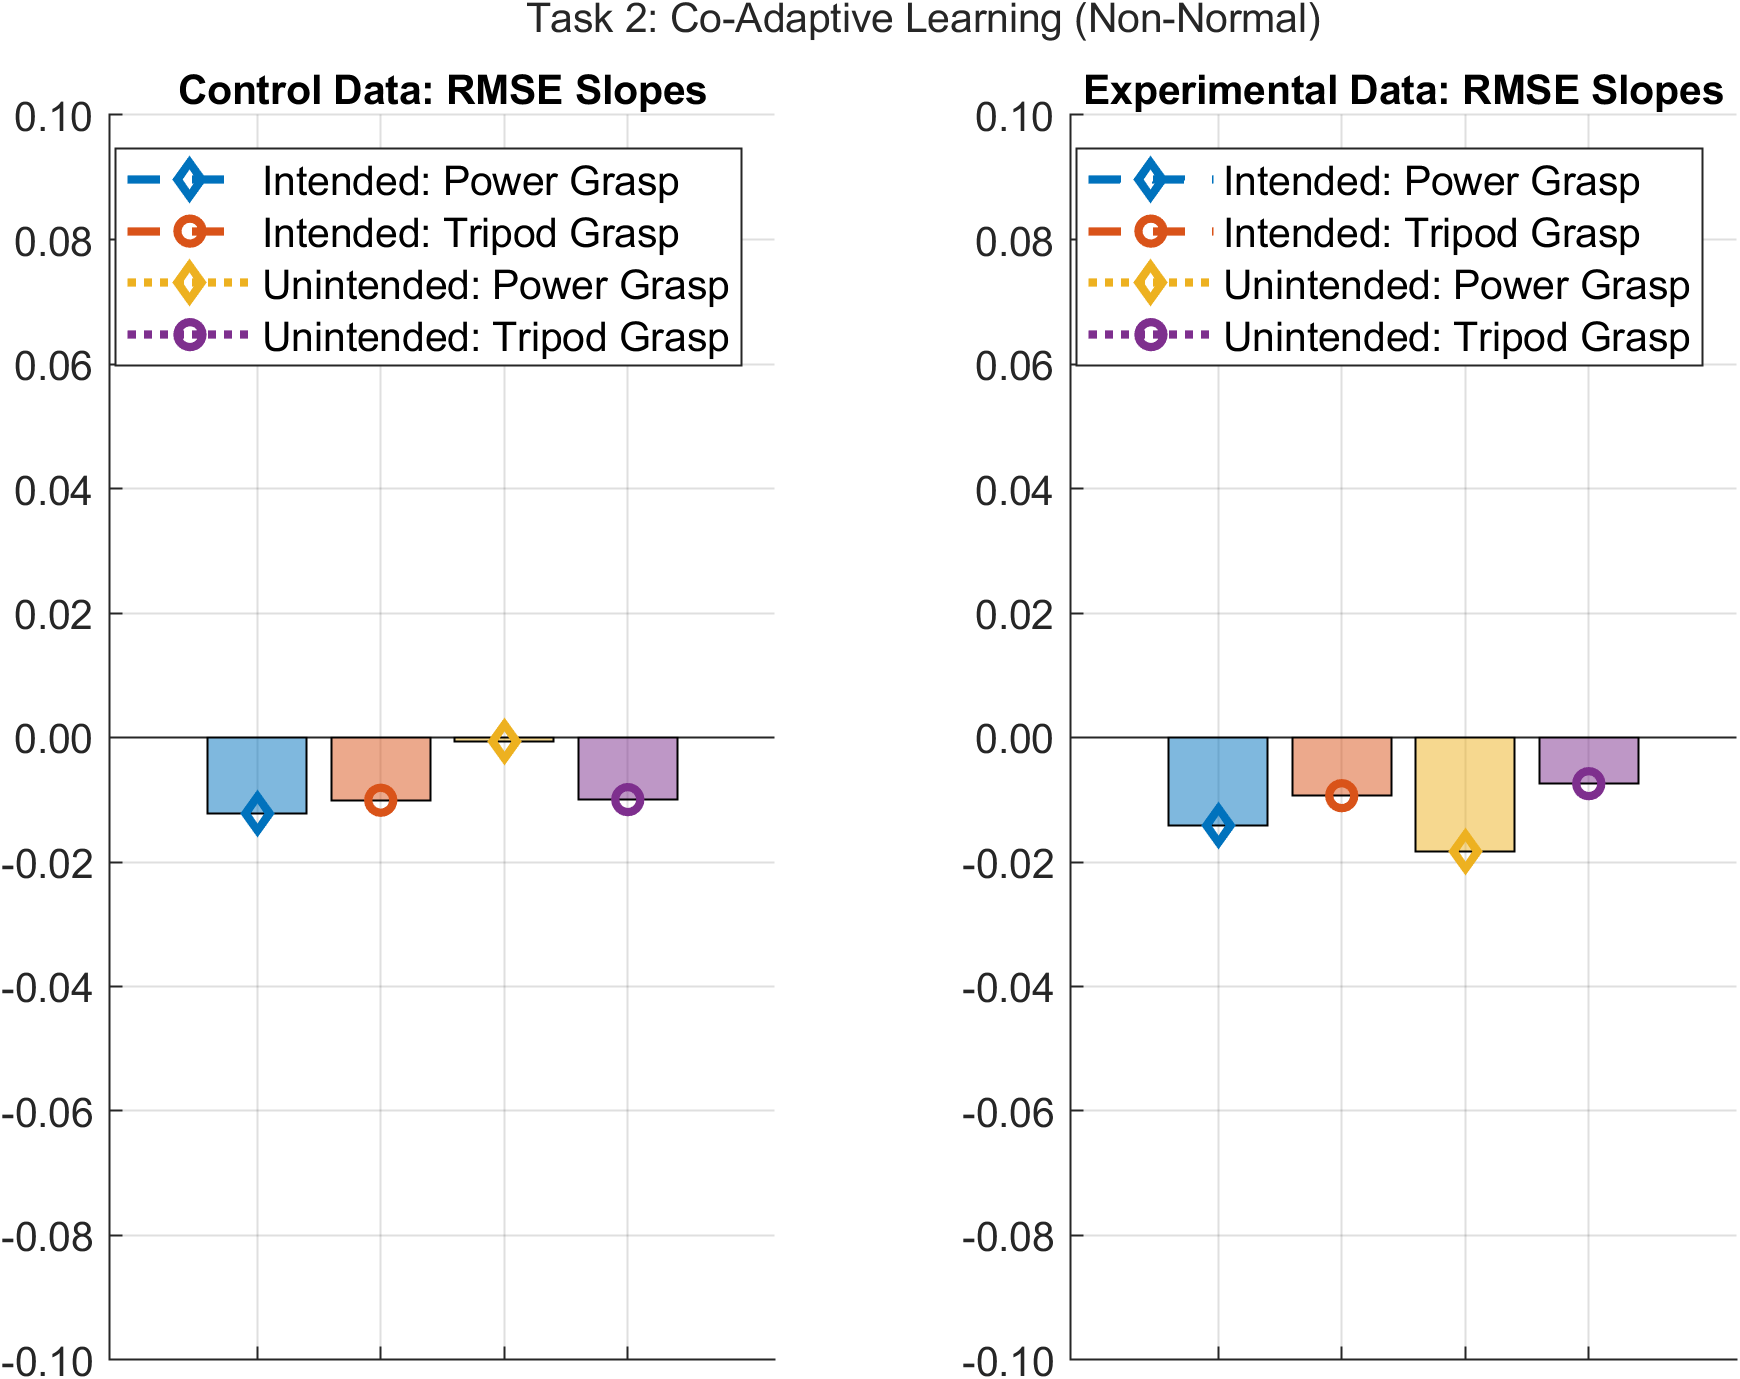
\includegraphics[width = \figWidth]{t2-bar-xnorm.png}
    \end{figure}
    \begin{figure}
        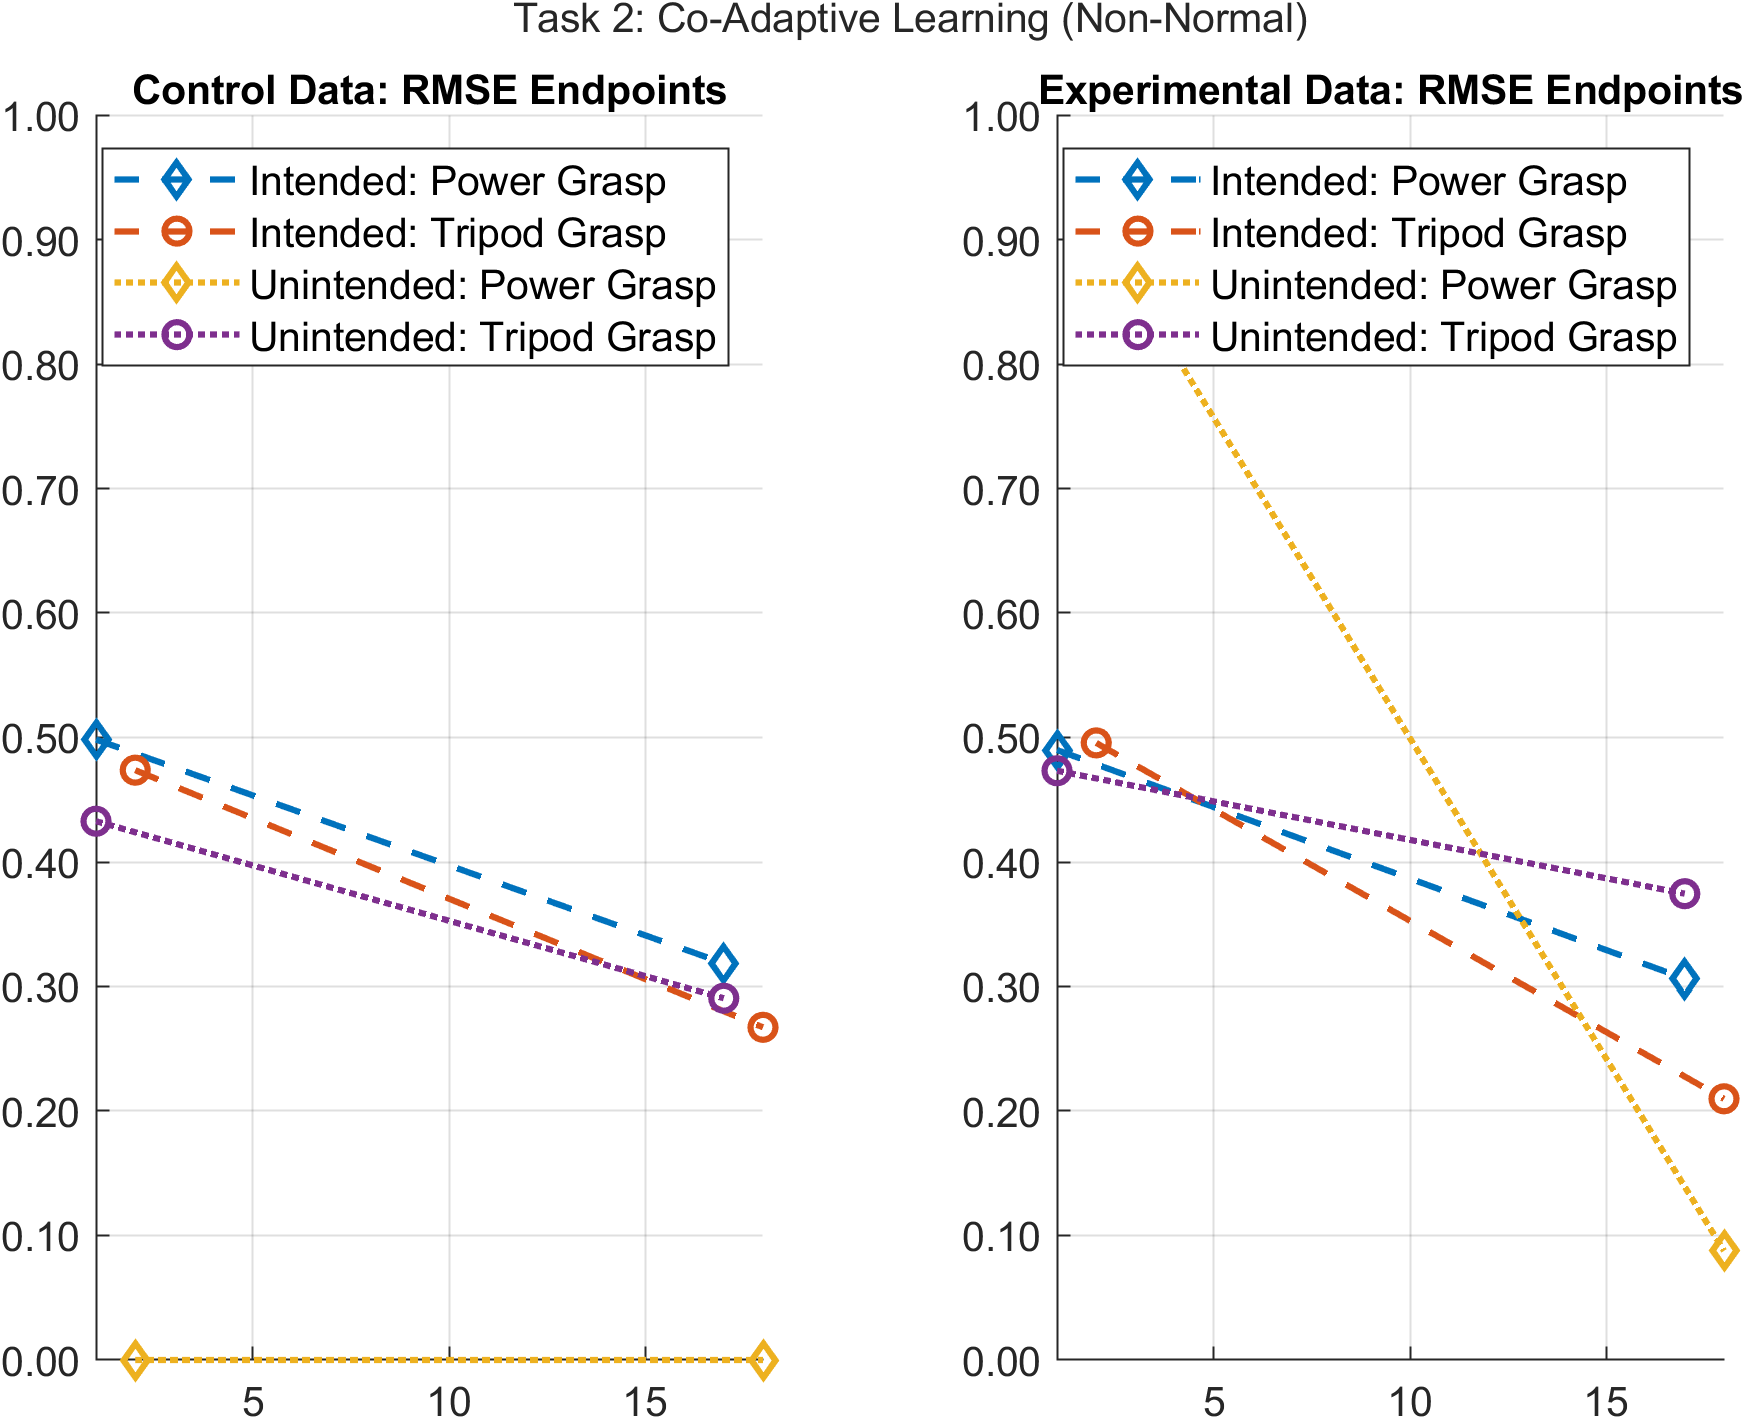
\includegraphics[width = \figWidth]{t2-spaghetti-xnorm.png}
    \end{figure}
    \newpage \clearpage
    %%%%%%%%%%%%%%%%%%%
    \begin{landscape}
    \begin{figure}
        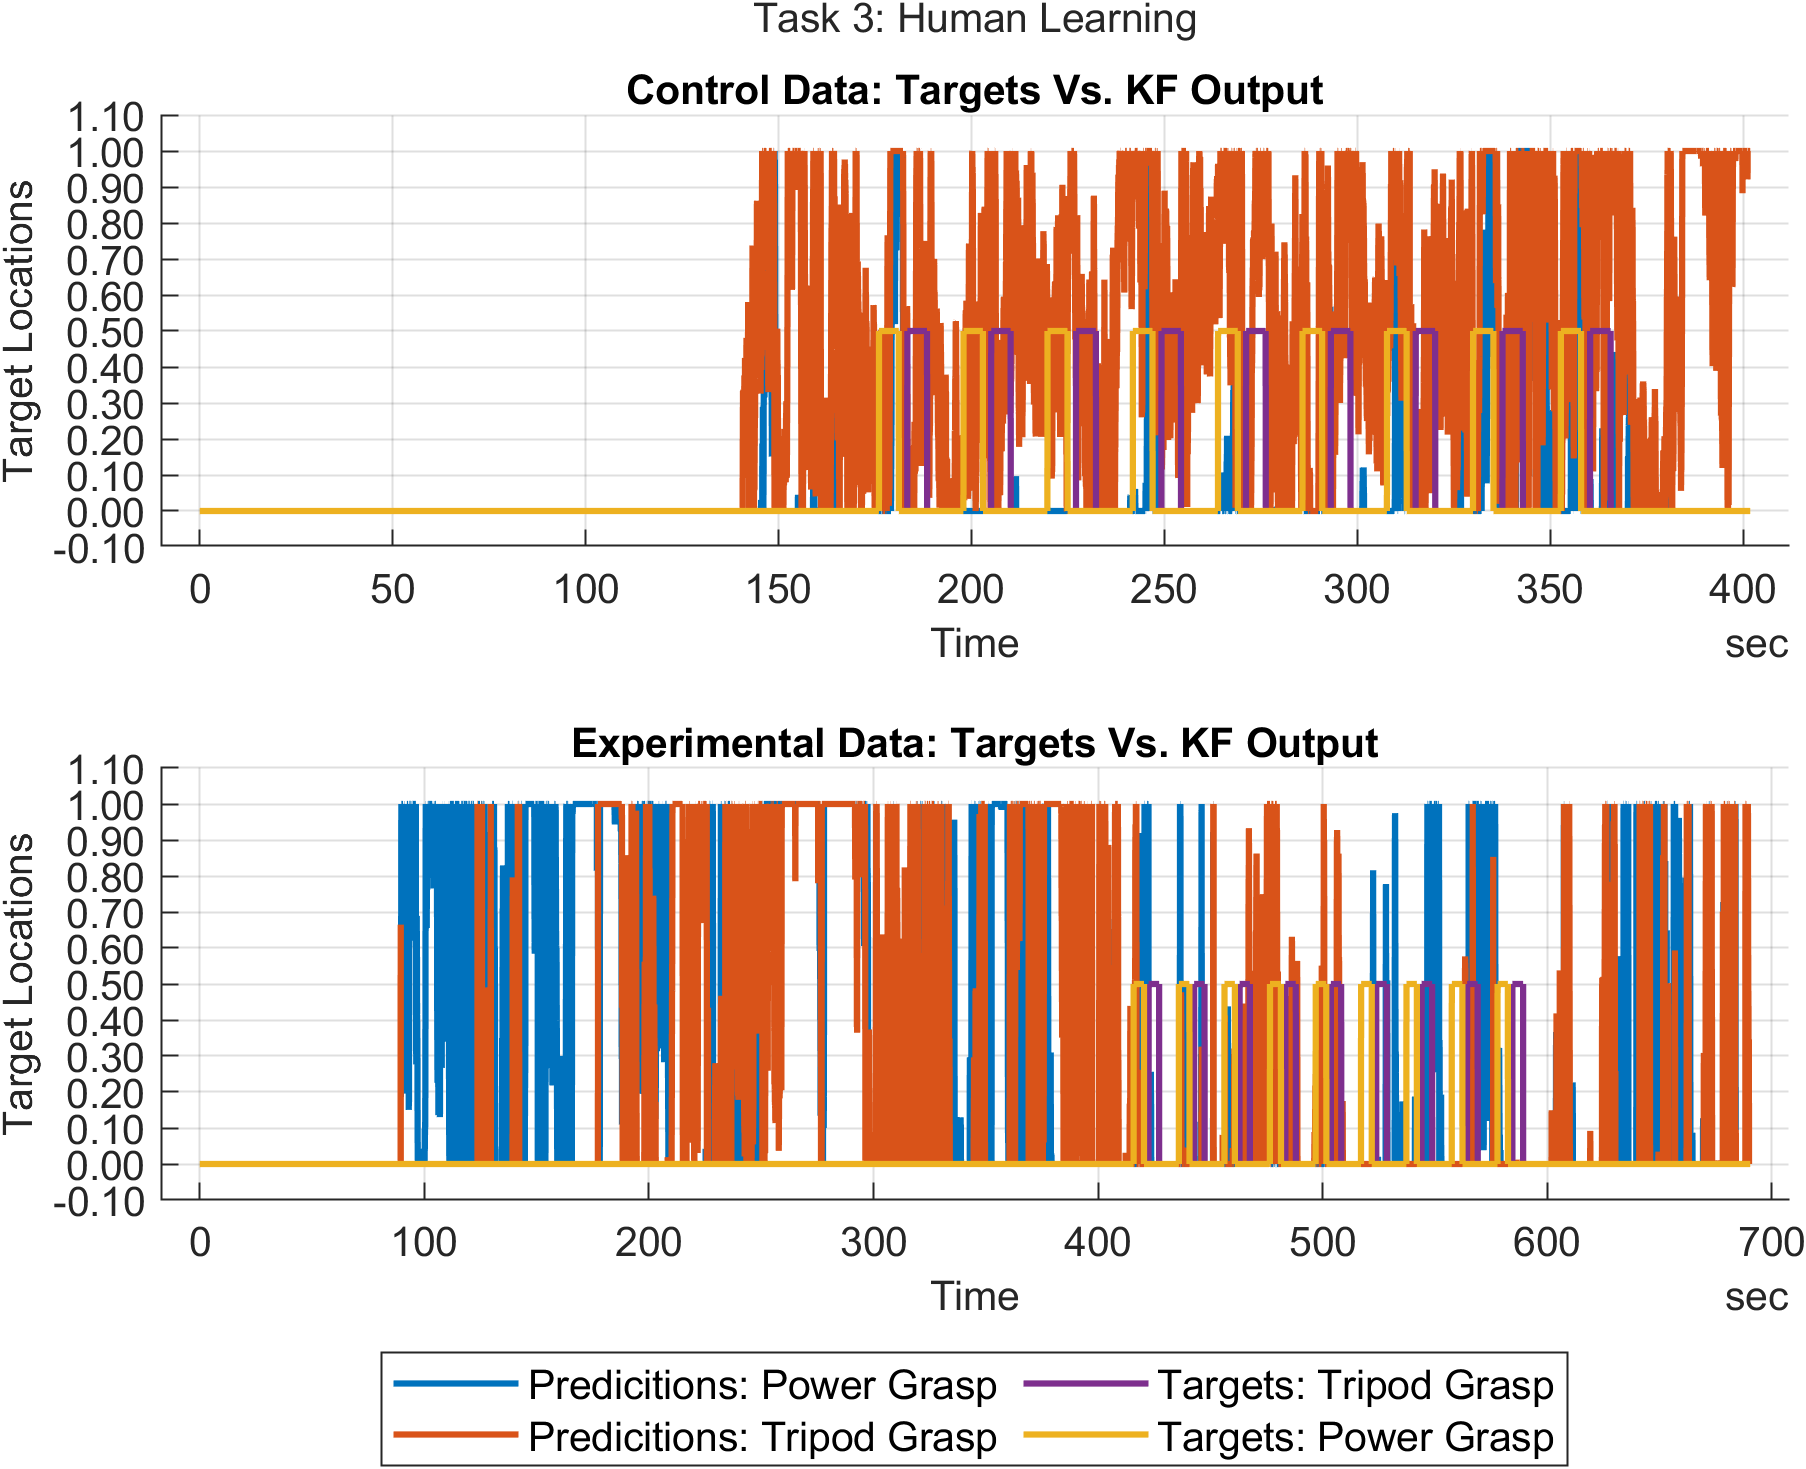
\includegraphics[width = \figWidthLarge]{t3-kf-out.png}
    \end{figure}
    \end{landscape}
    \newpage \clearpage
    \begin{figure}
        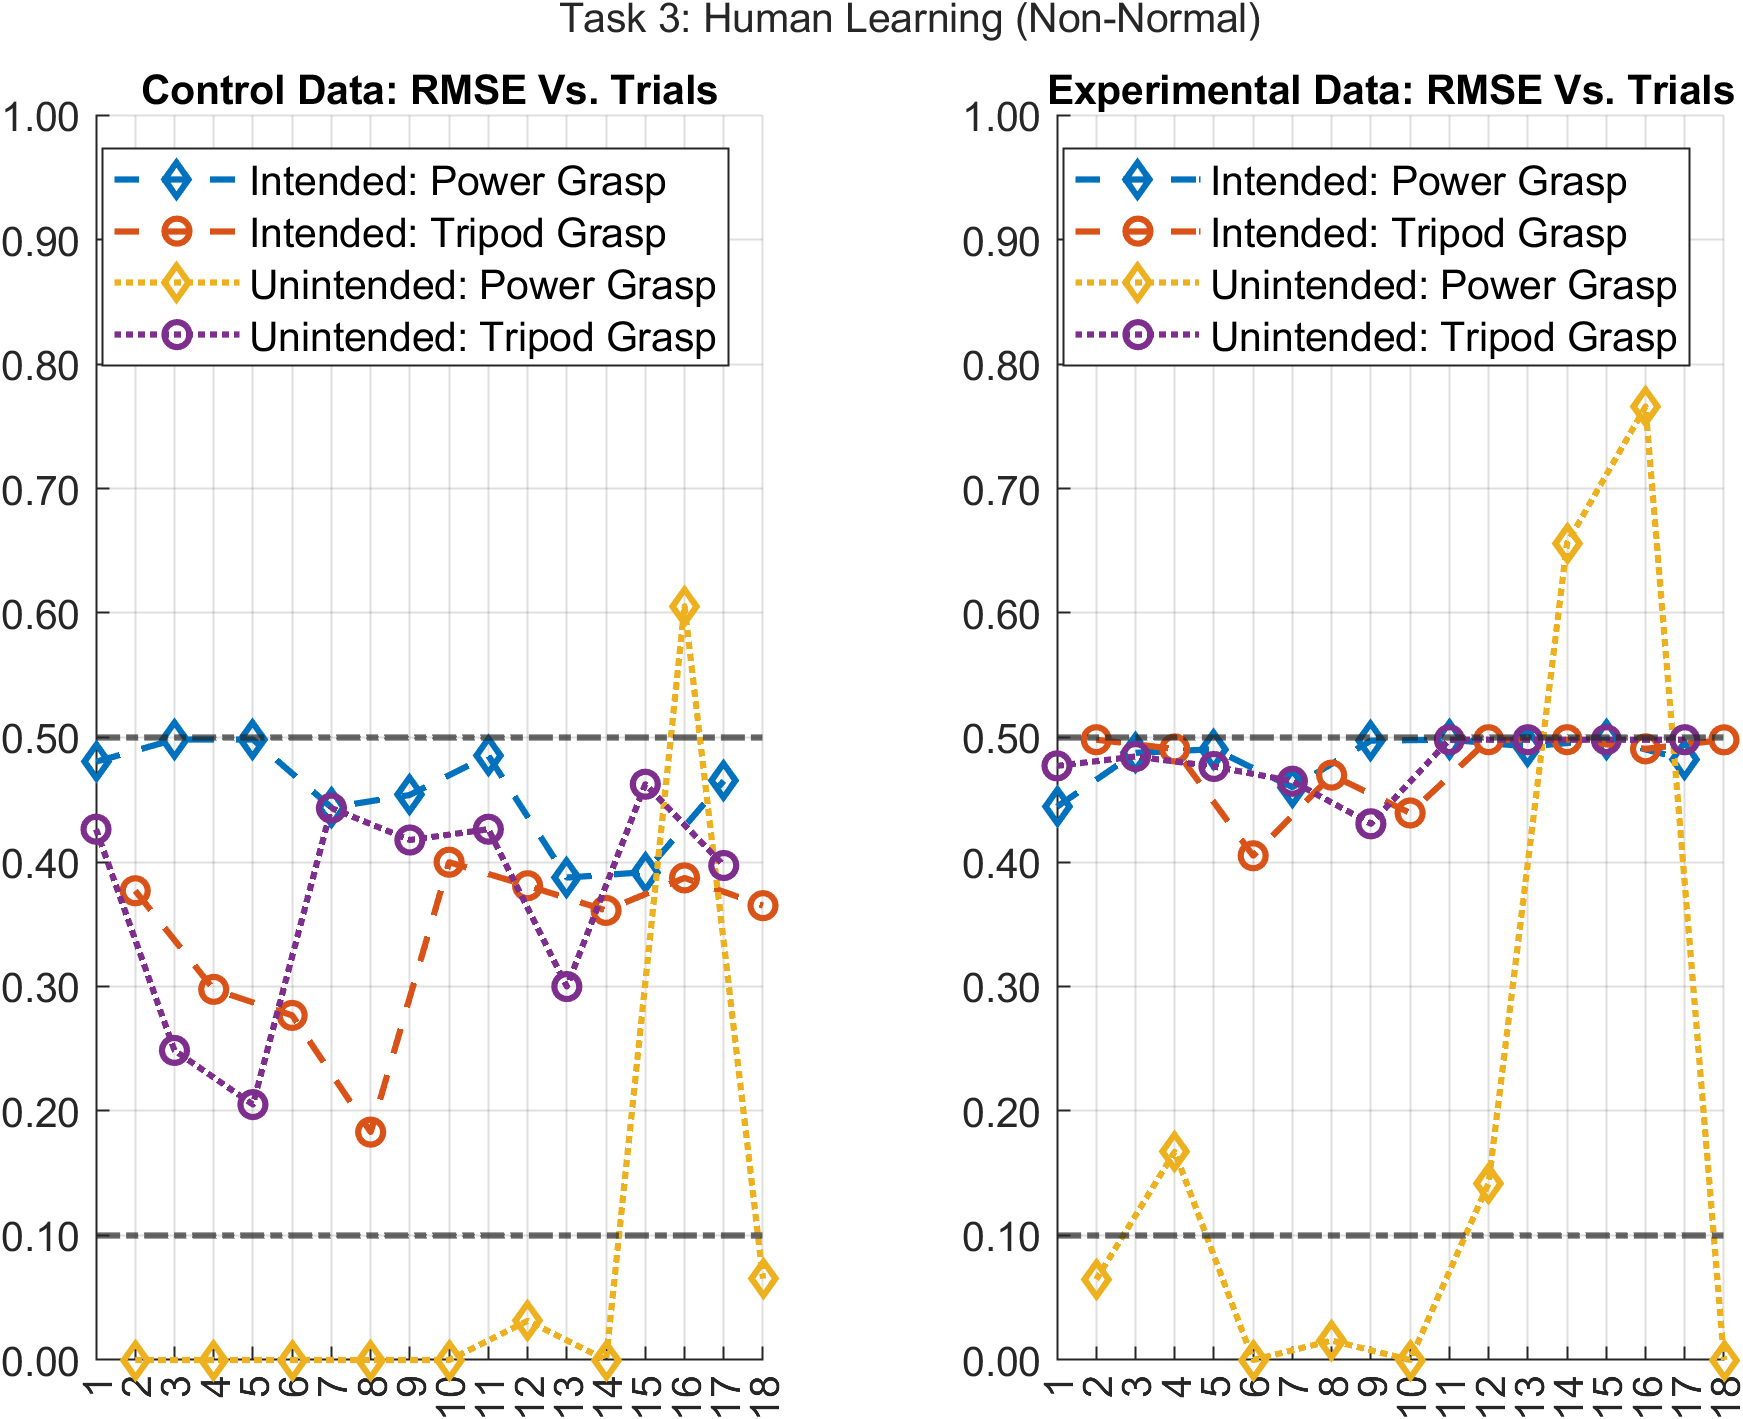
\includegraphics[width = \figWidth]{t3-rmse-xnorm.png}
    \end{figure}
    \begin{figure}
        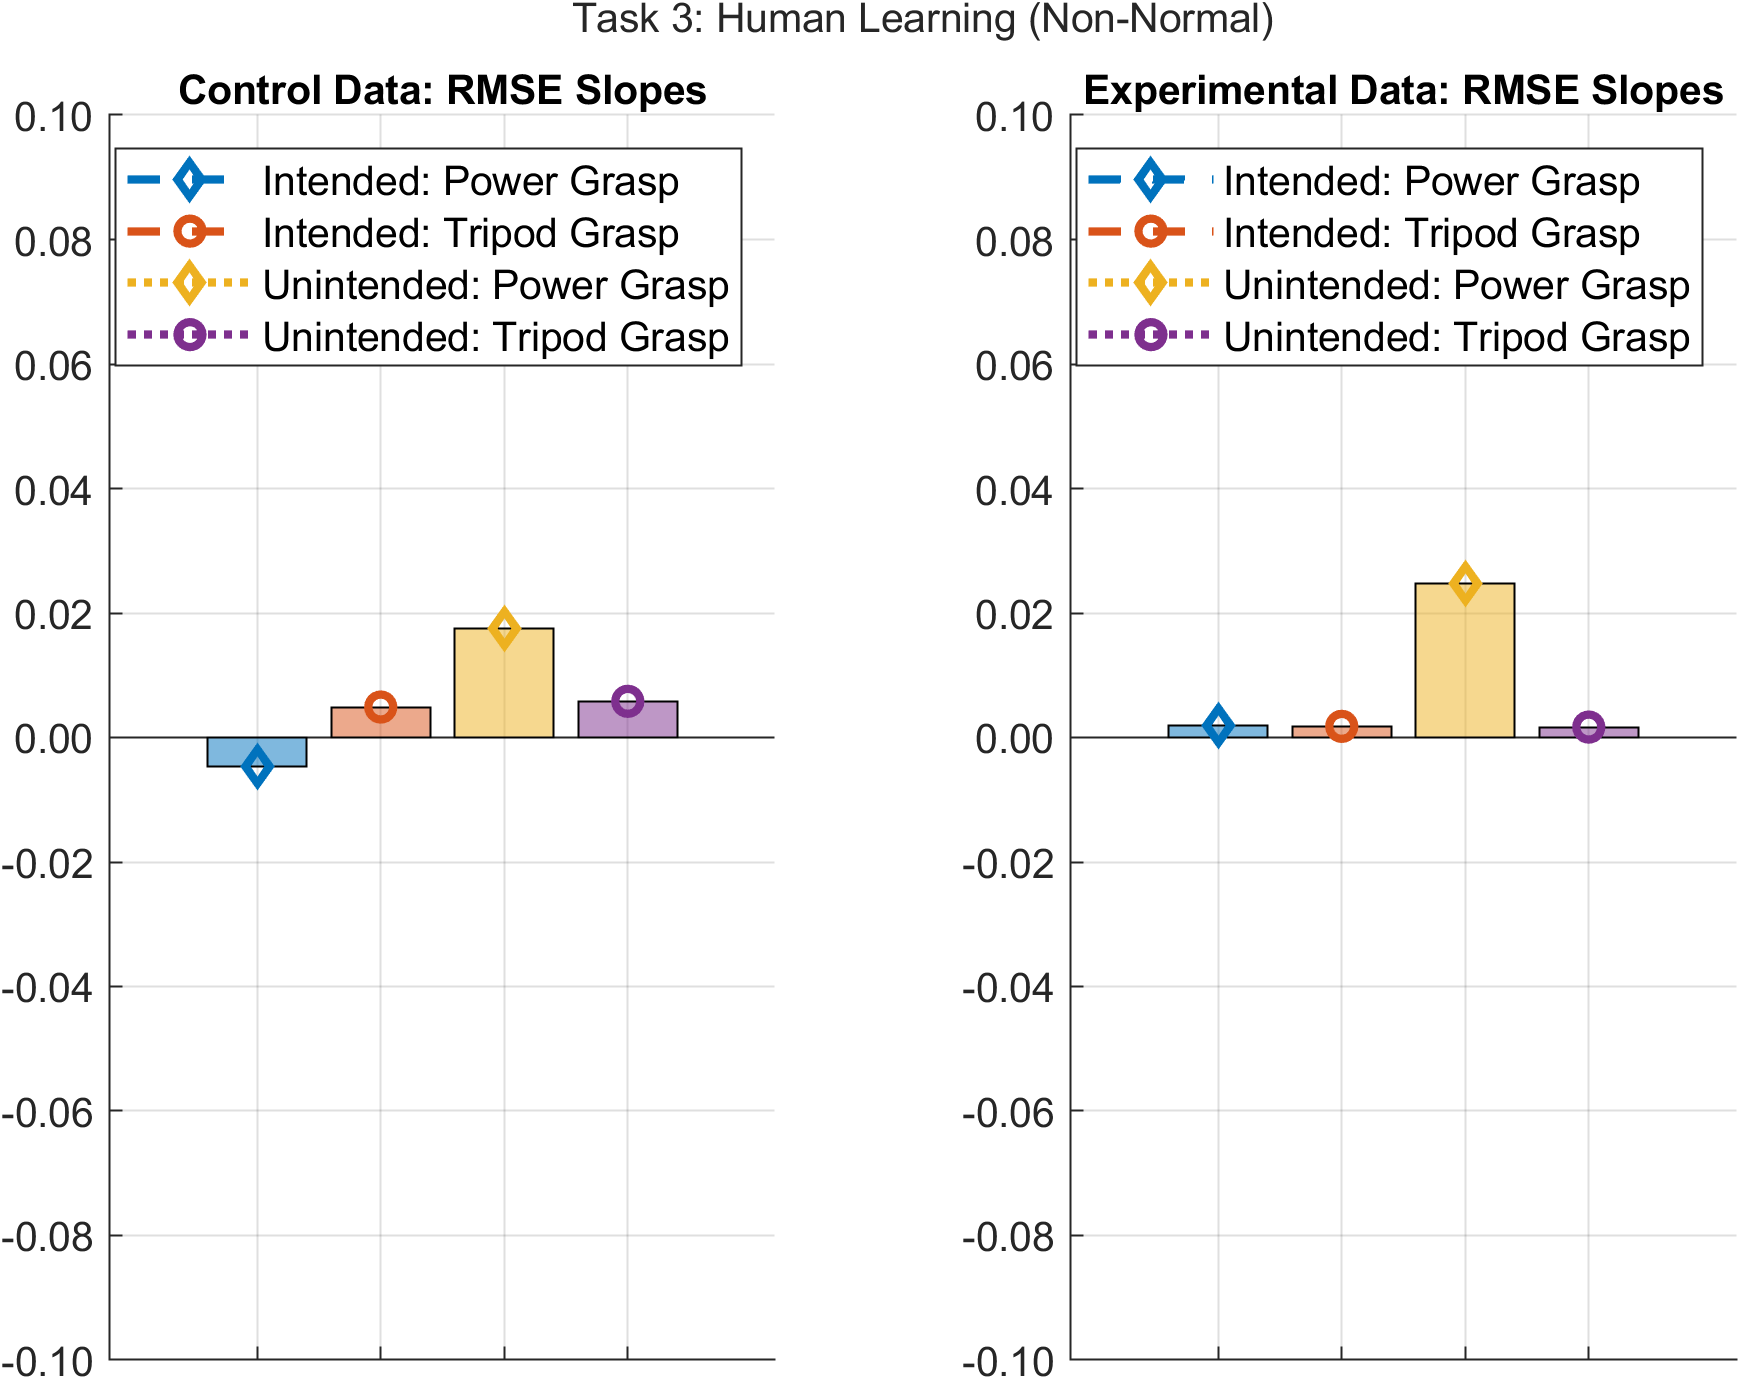
\includegraphics[width = \figWidth]{t3-bar-xnorm.png}
    \end{figure}
    \begin{figure}
        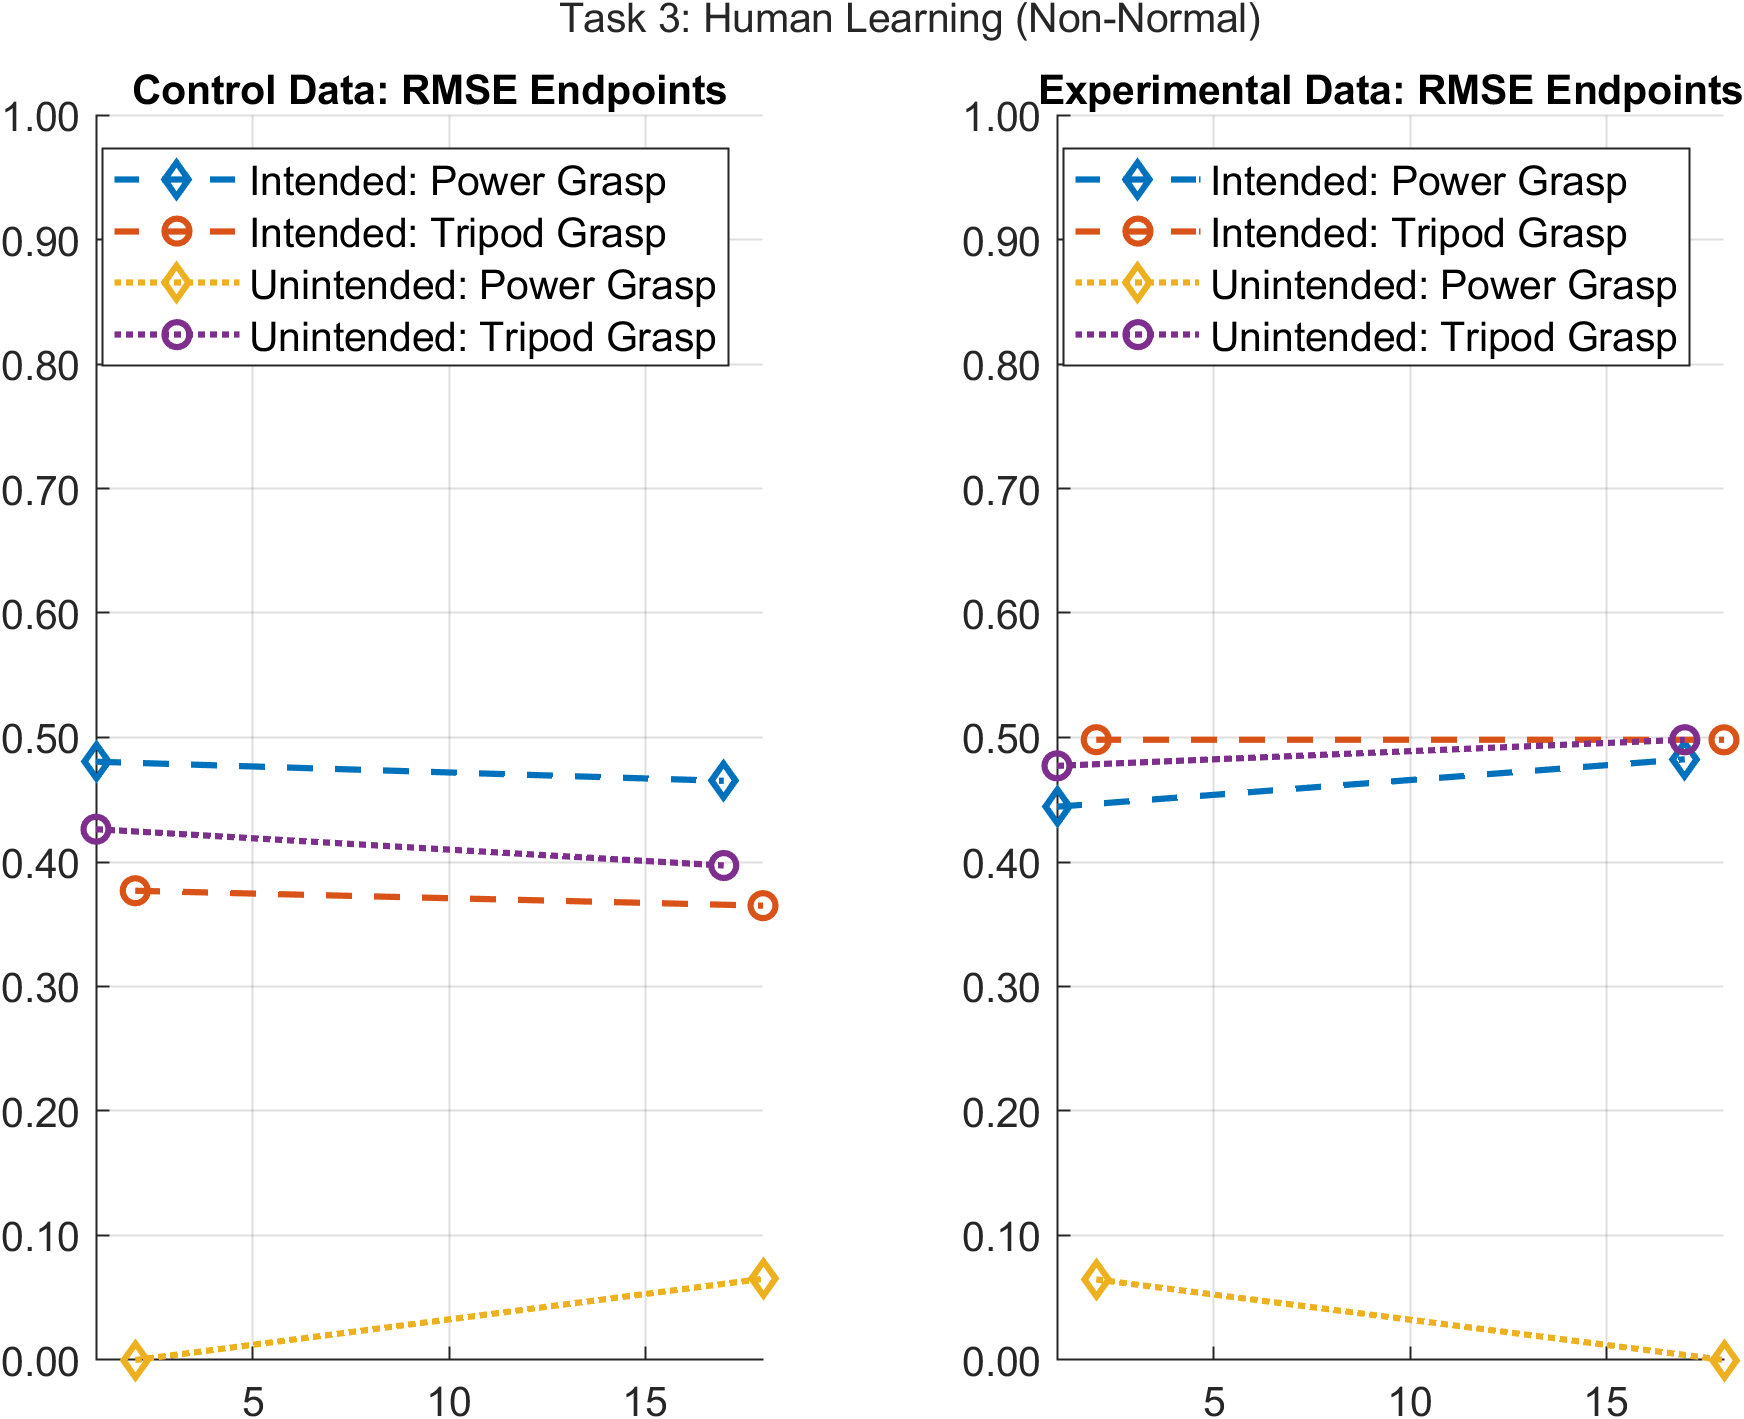
\includegraphics[width = \figWidth]{t3-spaghetti-xnorm.png}
    \end{figure}
\end{document}